\documentclass[border=2pt]{standalone}
\usepackage{pgfplots}\pgfplotsset{compat=1.18}\usepackage{amsmath}
\begin{document}
  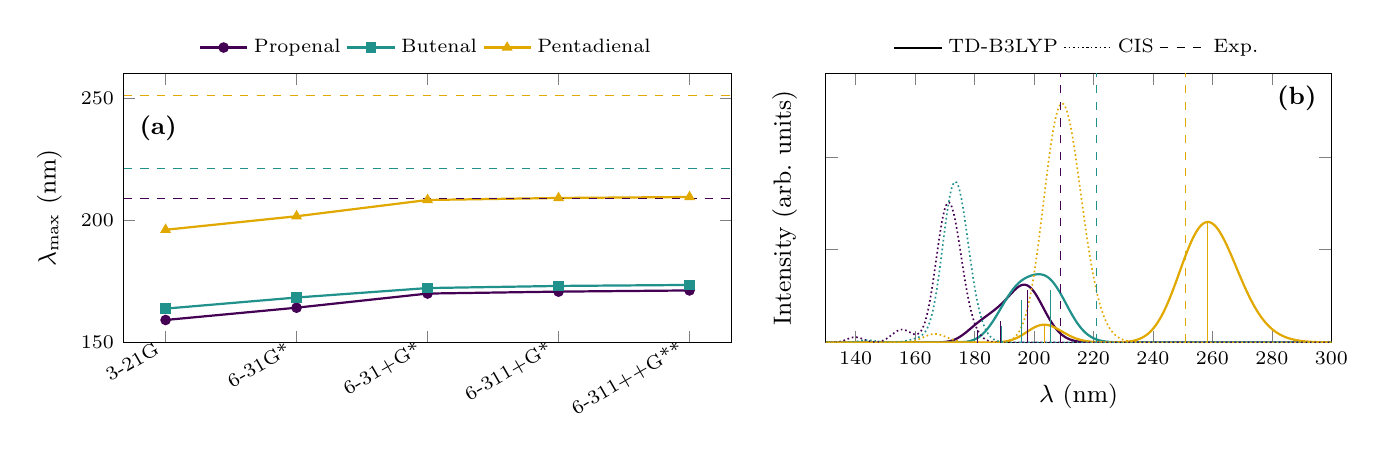
\begin{tikzpicture}
    \definecolor{c1}{HTML}{440154}
    \definecolor{c2}{HTML}{21918C}
    \definecolor{c3}{HTML}{E1A800}
    \begin{axis}[
        name=a, width=9.3cm, height=5cm,
        symbolic x coords={3-21G,6-31G*,6-31+G*,6-311+G*,6-311++G**},
        xtick=data, x tick label style={rotate=30, anchor=east, font=\scriptsize},
        ylabel={$\lambda_\mathrm{max}$ (nm)}, ymin=150, ymax=260,
        tick label style={font=\scriptsize}, label style={font=\small},
        tick align=inside, mark size=1.5pt, enlarge x limits=0.08,
        legend style={font=\scriptsize, draw=none, fill=none,
                      at={(0.5,1.02)}, anchor=south, legend columns=3},
        legend cell align=left]
      \addplot[c1, thick, mark=*] coordinates {(3-21G,159.21) (6-31G*,164.23)
        (6-31+G*,170.01) (6-311+G*,170.80) (6-311++G**,171.28)};
      \addplot[c2, thick, mark=square*] coordinates {(3-21G,163.86) (6-31G*,168.39)
        (6-31+G*,172.26) (6-311+G*,173.12) (6-311++G**,173.53)};
      \addplot[c3, thick, mark=triangle*] coordinates {(3-21G,196.08) (6-31G*,201.60)
        (6-31+G*,208.25) (6-311+G*,209.07) (6-311++G**,209.47)};
      \legend{Propenal, Butenal, Pentadienal}
      \draw[c1, dashed] (rel axis cs:0,0.536) -- (rel axis cs:1,0.536);
      \draw[c2, dashed] (rel axis cs:0,0.645) -- (rel axis cs:1,0.645);
      \draw[c3, dashed] (rel axis cs:0,0.918) -- (rel axis cs:1,0.918);
      \node[font=\small\bfseries, anchor=north west] at (rel axis cs:0.01,0.88) {(a)};
    \end{axis}
    \begin{axis}[
        at={(a.east)}, anchor=west, xshift=1.2cm,
        width=8cm, height=5cm,
        xlabel={$\lambda$ (nm)}, ylabel={Intensity (arb.\ units)},
        xmin=130, xmax=300, ymin=0, ymax=1.45, yticklabels={},
        tick label style={font=\scriptsize}, label style={font=\small},
        tick align=inside,
        legend style={font=\scriptsize, draw=none, fill=none,
                      at={(0.5,1.02)}, anchor=south, legend columns=3}]
      \addlegendimage{black, thick}\addlegendentry{TD-B3LYP}
      \addlegendimage{black, densely dotted, semithick}\addlegendentry{CIS}
      \addlegendimage{black, dashed}\addlegendentry{Exp.}
      \addplot[c1, thick, domain=130:300, samples=341] {0.2804*exp(-((1239.84/x-6.2664)/0.25)^2) + 0.1185*exp(-((1239.84/x-6.5743)/0.25)^2) + 0.07*exp(-((1239.84/x-6.8473)/0.25)^2)};
      \addplot[c2, thick, domain=130:300, samples=341] {0.2832*exp(-((1239.84/x-6.03)/0.25)^2) + 0.2278*exp(-((1239.84/x-6.329)/0.25)^2) + 0.0886*exp(-((1239.84/x-6.5546)/0.25)^2)};
      \addplot[c3, thick, domain=130:300, samples=341] {0.6492*exp(-((1239.84/x-4.7971)/0.25)^2) + 0.096*exp(-((1239.84/x-6.0939)/0.25)^2)};
      \addplot[c1, densely dotted, semithick, domain=130:300, samples=341] {0.755*exp(-((1239.84/x-7.2386)/0.25)^2) + 0.0697*exp(-((1239.84/x-7.9683)/0.25)^2) + 0.0288*exp(-((1239.84/x-8.8687)/0.25)^2)};
      \addplot[c2, densely dotted, semithick, domain=130:300, samples=341] {0.866*exp(-((1239.84/x-7.1448)/0.25)^2) + 0.022*exp(-((1239.84/x-7.6596)/0.25)^2) + 0.0123*exp(-((1239.84/x-8.617)/0.25)^2)};
      \addplot[c3, densely dotted, semithick, domain=130:300, samples=341] {1.2881*exp(-((1239.84/x-5.9191)/0.25)^2) + 0.0462*exp(-((1239.84/x-7.4395)/0.25)^2)};
      \addplot[c1, ycomb, thin, mark=none] coordinates {(197.86,0.2804) (188.59,0.1185) (181.07,0.07)};
      \addplot[c2, ycomb, thin, mark=none] coordinates {(205.61,0.2832) (195.90,0.2278) (189.16,0.0886)};
      \addplot[c3, ycomb, thin, mark=none] coordinates {(258.45,0.6492) (203.45,0.096)};
      \draw[c1, dashed] (axis cs:209,0) -- (axis cs:209,1.45);
      \draw[c2, dashed] (axis cs:221,0) -- (axis cs:221,1.45);
      \draw[c3, dashed] (axis cs:251,0) -- (axis cs:251,1.45);
      \node[font=\small\bfseries, anchor=north east] at (rel axis cs:0.99,0.99) {(b)};
    \end{axis}
  \end{tikzpicture}
\end{document}
